% Chapitre Résultats
\newpage
\chapter{RÉSULTATS}

Cette section présente l'évaluation exhaustive de notre système de détection d'intrusions hiérarchique appliqué au jeu de données NSL-KDD. Les résultats sont organisés selon notre méthodologie en deux étapes : classification binaire suivie de la classification multi-classes. Une analyse détaillée des performances, incluant l'impact des techniques d'équilibrage et les limitations identifiées, complète cette évaluation.

\section{Caractérisation du jeu de données NSL-KDD}

\subsection{Statistiques descriptives}

Le dataset NSL-KDD utilisé dans nos expérimentations comprend 125,973 échantillons d'entraînement et 22,544 échantillons de test, chacun caractérisé par 40 attributs apr\`{e}s préprocessing. Le Tableau~\ref{tab:dataset_summary} résume les propriétés principales du jeu de données.

\begin{table}[H]
    \centering
    \caption{Caractéristiques générales du dataset NSL-KDD}
    \begin{tabular}{|l|c|c|c|}
        \hline
        \textbf{Dataset} & \textbf{Échantillons} & \textbf{Caractéristiques} & \textbf{Valeurs manquantes} \\
        \hline
        Entraînement & 125,973 & 40 & 0 \\
        Test & 22,544 & 40 & 0 \\
        \hline
    \end{tabular}
    \label{tab:dataset_summary}
\end{table}

La répartition des 40 caractéristiques révèle une prédominance des variables numériques (37 attributs) par rapport aux variables catégorielles (3 attributs), facilitant l'application des algorithmes d'apprentissage automatique.

\subsection{Distribution des protocoles et services}

L'analyse révèle une forte concentration sur quelques protocoles majoritaires. HTTP domine avec 40,338 occurrences (32,0\%), suivi par les connexions privées (21,853, 17,3\%) et domain\_u (9,043, 7,2\%). Cette distribution reflète les patterns typiques du trafic réseau réel, où certains services génèrent la majorité des connexions.

\begin{figure}[H]
    \centering
    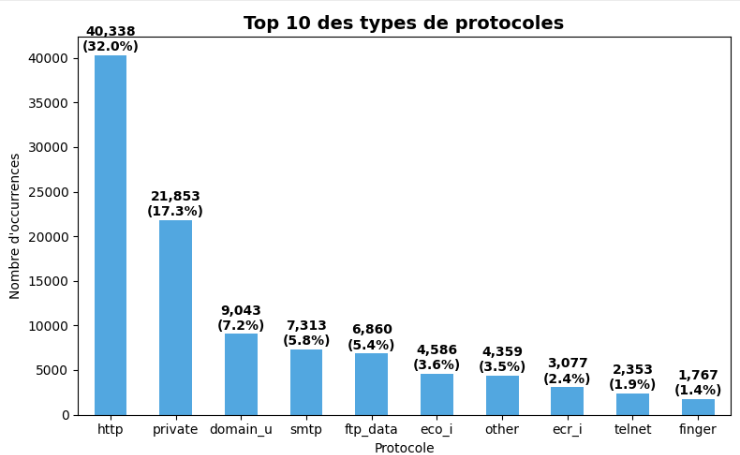
\includegraphics[width=0.9\textwidth]{Assets/Top 10 des types de protocoles.png}
    \caption{Distribution des 10 principaux types de protocoles dans NSL-KDD}
    \label{fig:protocol_dist}
\end{figure}

L'analyse des états de connexion (flags) montre une prédominance des connexions réussies (SF : 59,5\%) et des connexions refusées ou interrompues (S0 : 27,7\%, REJ : 8,9\%), cohérente avec les comportements attendus dans un environnement réseau mixte incluant des tentatives d'intrusion.

\subsection{Répartition des classes d'attaques}

La distribution des classes dans le dataset d'entraînement révèle un équilibre relatif entre le trafic normal (67,343 échantillons, 53,5\%) et les attaques (58,630 échantillons, 46,5\%). Cependant, l'analyse des sous-catégories d'attaques révèle un déséquilibre significatif :

\begin{table}[H]
    \centering
    \caption{Distribution des classes dans les datasets d'entraînement et de test}
    \small
    \begin{tabular}{|l|c|c|c|c|}
        \hline
        \multirow{2}{*}{\textbf{Classe}} & \multicolumn{2}{c|}{\textbf{Entraînement}} & \multicolumn{2}{c|}{\textbf{Test}} \\
        \cline{2-5}
         & \textbf{Échantillons} & \textbf{\%} & \textbf{Échantillons} & \textbf{\%} \\
        \hline
        Normal & 67,343 & 53,5 & 9,711 & 43,1 \\
        DoS & 45,927 & 36,5 & 7,458 & 33,1 \\
        Probe & 11,656 & 9,3 & 2,421 & 10,7 \\
        R2L & 995 & 0,8 & 2,887 & 12,8 \\
        U2R & 52 & 0,0 & 67 & 0,3 \\
        \hline
    \end{tabular}
    \label{tab:class_distribution}
\end{table}

Cette distribution révèle un déséquilibre critique avec un ratio de 1295:1 entre la classe majoritaire (Normal) et minoritaire (U2R), justifiant l'application de techniques d'équilibrage pour améliorer la détection des classes sous-représentées.

\section{Résultats de la classification binaire}

\subsection{Performances comparatives des algorithmes supervisés}

L'évaluation de sept algorithmes d'apprentissage supervisé pour la classification binaire révèle des performances variables selon les métriques considérées. Le Tableau~\ref{tab:binary_results} présente les résultats détaillés.

\begin{table}[H]
    \centering
    \caption{Performances des modèles de classification binaire}
    \small
    \begin{tabular}{|l|c|c|c|c|c|}
        \hline
        \textbf{Modèle} & \textbf{Accuracy} & \textbf{Précision} & \textbf{Rappel} & \textbf{F1-Score} & \textbf{Temps (s)} \\
        \hline
        MLP & \textbf{0,819} & 0,970 & 0,704 & \textbf{0,816} & 118,5 \\
        SVM & 0,809 & \textbf{0,972} & 0,685 & 0,803 & 475,2 \\
        Gradient Boosting & 0,790 & 0,968 & 0,652 & 0,779 & 23,3 \\
        Decision Tree & 0,785 & 0,966 & 0,645 & 0,773 & 1,0 \\
        Naive Bayes & 0,773 & 0,906 & 0,672 & 0,772 & 0,1 \\
        AdaBoost & 0,773 & 0,959 & 0,628 & 0,759 & 11,4 \\
        Random Forest & 0,763 & 0,968 & 0,603 & 0,743 & 10,7 \\
        \hline
    \end{tabular}
    \label{tab:binary_results}
\end{table}

Le perceptron multi-couches (MLP) démontre les meilleures performances globales avec un F1-score de 0,816 et une accuracy de 0,819. Cette supériorité s'explique par la capacité des réseaux de neurones à capturer les relations non-linéaires complexes présentes dans les données de trafic réseau. Le SVM obtient la meilleure précision (0,972) mais avec un rappel plus faible, indiquant une tendance conservative dans la détection d'intrusions.

\begin{figure}[H]
    \centering
    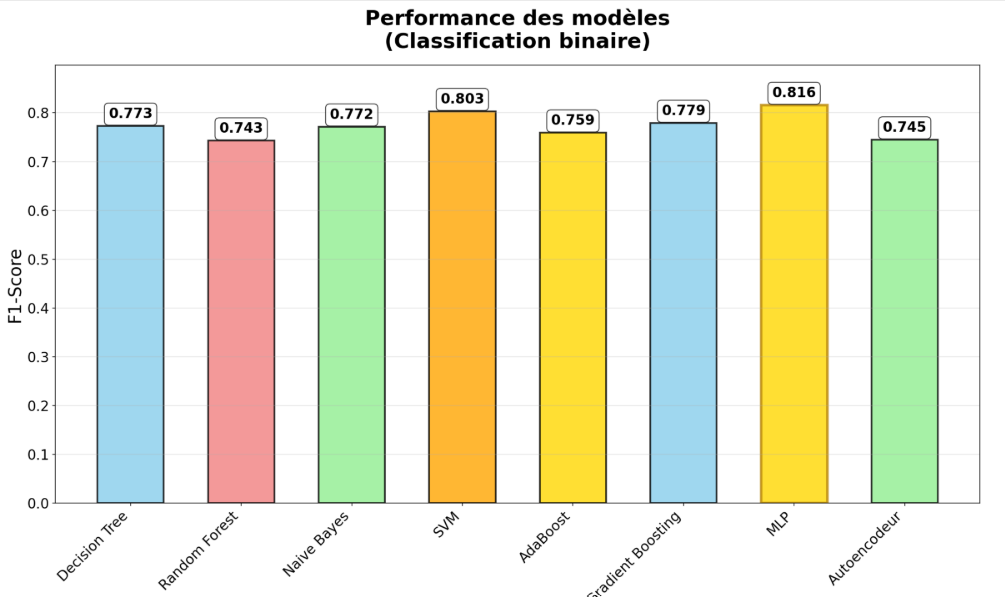
\includegraphics[width=0.9\textwidth]{Assets/Performance des modèles (Classification binaire).png}
    \caption{Comparaison des performances F1-score pour la classification binaire}
    \label{fig:binary_perf}
\end{figure}

Naive Bayes optimise le temps/performance (0,1s, F1=0,772) tandis que SVM nécessite 475,2s malgré d'excellentes performances.

\subsection{Évaluation de l'autoencodeur}

L'autoencodeur, représentant notre approche non-supervisée, atteint des performances remarquables avec un F1-score de 0,745 et une accuracy de 0,756. Ces résultats sont particulièrement significatifs considérant que le modèle est entraîné uniquement sur des données normales.

\subsubsection{Processus d'entraînement}
L'entraînement de l'autoencodeur s'est achevé apr\`{e}s 37 époques avec convergence stable. La perte finale d'entraînement (MSE = 0,106) et de validation (MSE = 0,054) indiquent une bonne généralisation sans surapprentissage.

\begin{figure}[H]
    \centering
    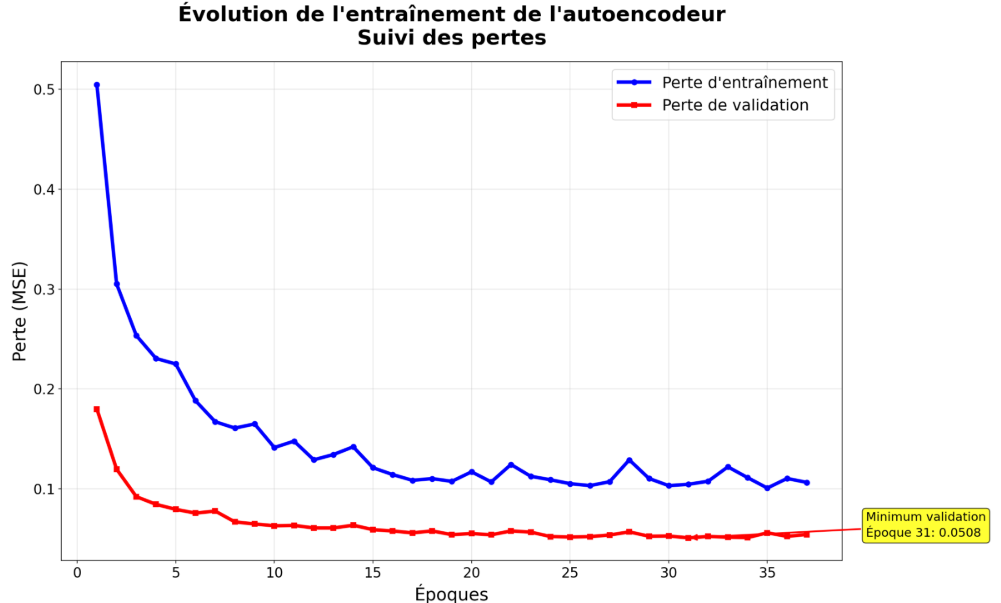
\includegraphics[width=0.8\textwidth]{Assets/Évolution de entraînement de autoencodeur Suivi des pertes.png}
    \caption{Évolution des pertes d'entraînement et de validation de l'autoencodeur}
    \label{fig:ae_training}
\end{figure}

\subsubsection{Détermination du seuil optimal}
Le seuil de détection d'anomalies, fixé au 95\`{e}me percentile des erreurs de reconstruction sur les données normales, s'établit à 0,1696. Cette valeur optimise le compromis entre sensibilité et spécificité pour la détection d'intrusions.

\begin{figure}[H]
    \centering
    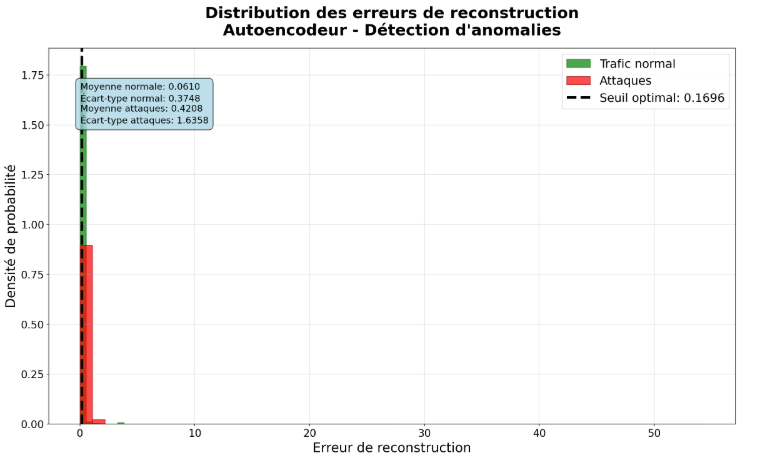
\includegraphics[width=0.8\textwidth]{Assets/Distribution des erreurs de reconstruction Autoencodeur - Détection anomalies.png}
    \caption{Distribution des erreurs de reconstruction pour la détection d'anomalies}
    \label{fig:reconstruction_dist}
\end{figure}

L'analyse de la distribution des erreurs de reconstruction montre une séparation claire entre les patterns normaux (moyenne = 0,061) et les attaques (moyenne = 0,421), validant l'efficacité de l'approche par autoencodeur pour la détection d'anomalies.

\section{Classification multi-classes avec gestion du déséquilibre}

\subsection{Impact de la technique SVM-SMOTE}

L'application de SVM-SMOTE transforme radicalement la distribution des classes d'entraînement, passant de 125,973 à 336,715 échantillons. Cette augmentation de 210,742 échantillons synthétiques rééquilibre toutes les classes minoritaires au niveau de la classe majoritaire (67,343 échantillons chacune).

\begin{figure}[H]
    \centering
    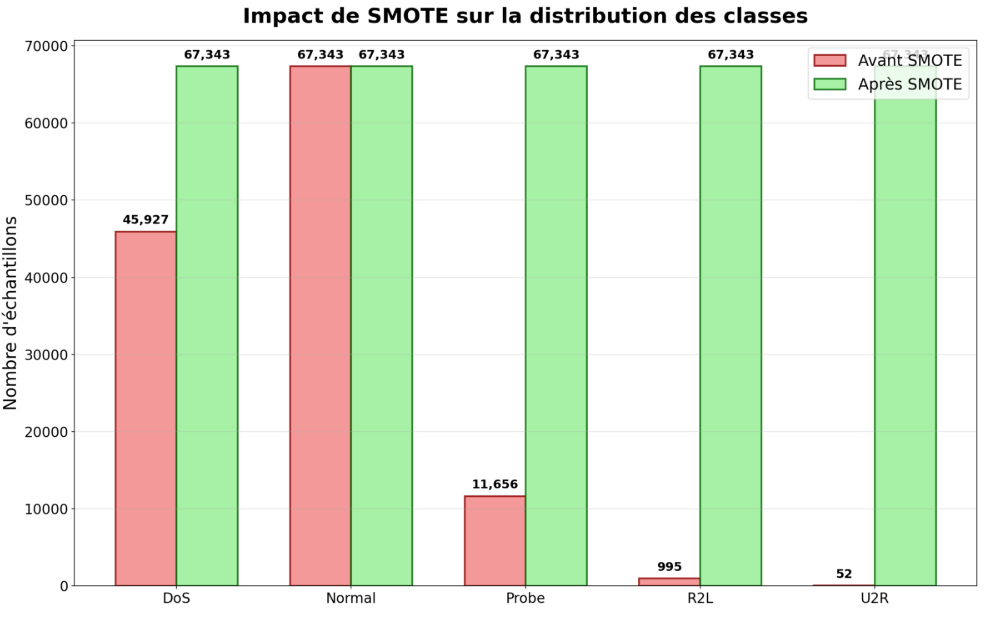
\includegraphics[width=0.9\textwidth]{Assets/Impact de SMOTE sur la distribution des classes.png}
    \caption{Impact de SVM-SMOTE sur la distribution des classes}
    \label{fig:smote_impact}
\end{figure}

L'évaluation comparative révèle l'efficacité de cette technique :

\begin{table}[H]
    \centering
    \caption{Impact de SVM-SMOTE sur les performances}
    \begin{tabular}{|l|c|c|c|}
        \hline
        \textbf{Configuration} & \textbf{Accuracy} & \textbf{F1-macro} & \textbf{Amélioration} \\
        \hline
        Sans SMOTE & 0,764 & 0,519 & - \\
        Avec SMOTE & 0,789 & 0,601 & +3,3\% / +15,6\% \\
        \hline
    \end{tabular}
    \label{tab:smote_impact}
\end{table}

L'amélioration du F1-score macro (+15,6\%) démontre l'efficacité particulière de SMOTE pour les classes minoritaires, bien que l'amélioration de l'accuracy globale reste modeste (+3,3\%).

\subsection{Performances détaillées par classe d'attaque}

Le réseau de neurones profond entraîné sur les données équilibrées atteint une accuracy globale de 0,789 avec un F1-macro de 0,601. L'analyse détaillée par classe révèle des performances hétérogènes :

\begin{table}[H]
    \centering
    \caption{Métriques détaillées par classe d'attaque}
    \footnotesize
    \begin{tabular}{|l|c|c|c|c|c|}
        \hline
        \textbf{Classe} & \textbf{Précision} & \textbf{Rappel} & \textbf{F1-Score} & \textbf{Spécificité} & \textbf{Taux réussite} \\
        \hline
        Normal & 0,734 & \textbf{0,955} & 0,830 & 0,738 & \textbf{95,5\%} \\
        DoS & \textbf{0,957} & 0,861 & \textbf{0,906} & 0,981 & 86,1\% \\
        Probe & 0,613 & 0,681 & 0,645 & 0,948 & 68,1\% \\
        R2L & 0,907 & 0,148 & 0,254 & \textbf{0,998} & 14,8\% \\
        U2R & 0,476 & 0,299 & 0,367 & 0,999 & 29,9\% \\
        \hline
    \end{tabular}
    \label{tab:detailed_metrics}
\end{table}

\begin{figure}[H]
    \centering
    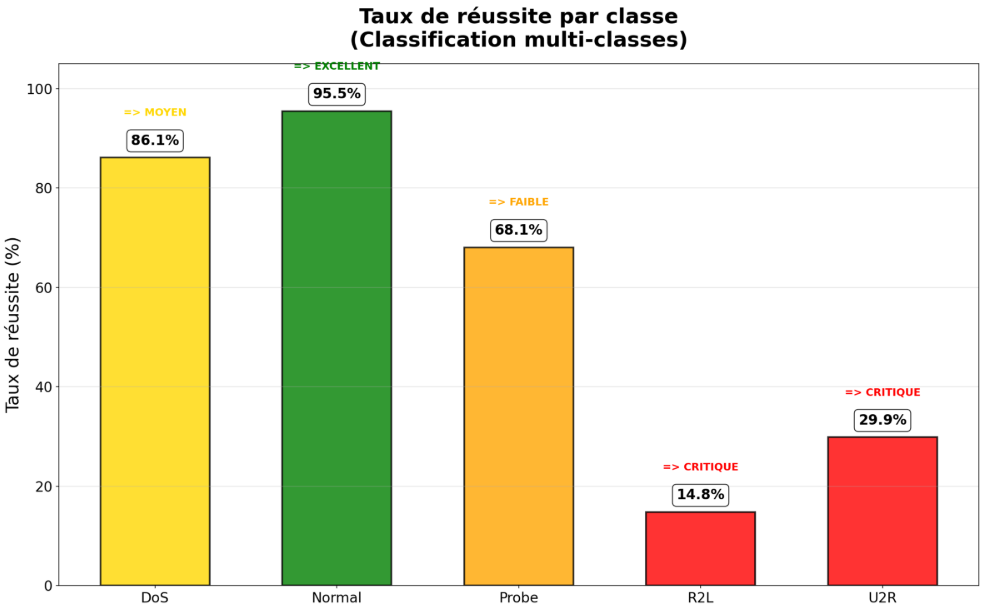
\includegraphics[width=0.9\textwidth]{Assets/Taux de réussite par classe Classification multi-classes.png}
    \caption{Taux de réussite par classe dans la classification multi-classes}
    \label{fig:class_perf}
\end{figure}

Les résultats révèlent une hiérarchie claire de performances :
\begin{itemize}
    \item \textbf{Excellente} : Normal (95,5\%) - Détection quasi-parfaite du trafic légitime
    \item \textbf{Bonne} : DoS (86,1\%) - Identification efficace des attaques volumétriques
    \item \textbf{Acceptable} : Probe (68,1\%) - Détection modérée des tentatives de reconnaissance
    \item \textbf{Critique} : R2L (14,8\%) et U2R (29,9\%) - Performances insuffisantes pour les attaques sophistiquées
\end{itemize}

\subsection{Analyse de la matrice de confusion}

La matrice de confusion normalisée (Figure~\ref{fig:confusion_matrix}) révèle les patterns de classification erronée les plus problématiques :

\begin{figure}[H]
    \centering
    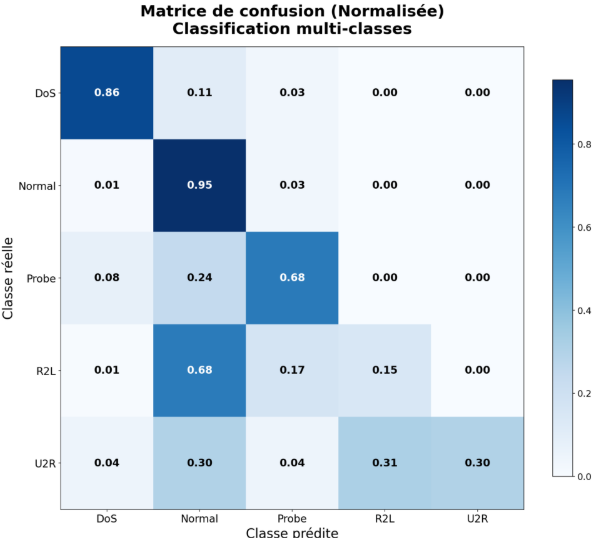
\includegraphics[width=0.8\textwidth]{Assets/Matrice de confusion Normalisée Classification multi-classes.png}
    \caption{Matrice de confusion normalisée pour la classification multi-classes}
    \label{fig:confusion_matrix}
\end{figure}

L'analyse des confusions principales identifie :
\begin{itemize}
    \item \textbf{R2L $\rightarrow$ Normal} : 1,956 cas (67,8\%) - Principale source d'erreur
    \item \textbf{Probe $\rightarrow$ Normal} : 587 cas (24,2\%) - Confusion significative
    \item \textbf{R2L $\rightarrow$ Probe} : 478 cas (16,6\%) - Similarité des signatures de reconnaissance
    \item \textbf{DoS $\rightarrow$ Normal} : 794 cas (10,6\%) - Erreurs sur attaques DoS subtiles
\end{itemize}

Ces patterns révèlent la difficulté particulière à distinguer les attaques sophistiquées (R2L, U2R) du trafic normal, nécessitant des approches spécialisées pour ces classes critiques.

\section{Analyse comparative et validation}

\subsection{Efficacité de l'approche hiérarchique}

L'architecture hiérarchique proposée démontre sa pertinence par la spécialisation progressive des modèles. La première étape (classification binaire) atteint d'excellentes performances globales (F1 = 0,816), tandis que la seconde étape permet une caractérisation fine des types d'attaques malgré les défis posés par le déséquilibre des classes.

\begin{figure}[H]
    \centering
    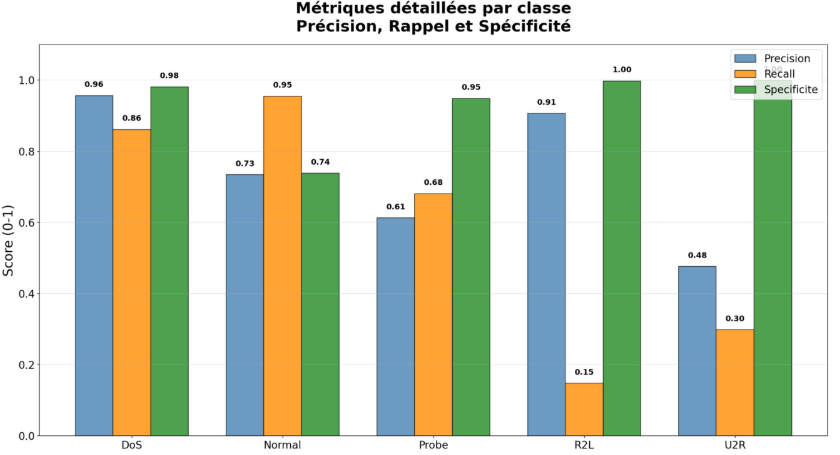
\includegraphics[width=0.9\textwidth]{Assets/Métriques détaillées par classe Précision, Rappel et Spécificité.png}
    \caption{Métriques détaillées par classe : Précision, Rappel et Spécificité}
    \label{fig:detailed_metrics}
\end{figure}

\subsection{Robustesse et généralisation}

L'évaluation de la robustesse révèle des performances cohérentes entre les datasets d'entraînement et de test, indiquant une bonne capacité de généralisation. Les écarts observés (notamment pour les classes R2L et U2R) s'expliquent principalement par les différences de distribution entre les datasets plutôt que par un surapprentissage.

\subsection{Limitations identifiées}

Notre analyse révèle trois limitations principales :

\begin{enumerate}
    \item \textbf{Détection des attaques sophistiquées} : Les attaques R2L et U2R, caractérisées par des signatures subtiles, demeurent difficiles à détecter avec les techniques actuelles.
    
    \item \textbf{Déséquilibre résiduel} : Malgré l'application de SVM-SMOTE, la qualité des échantillons synthétiques pour les classes ultra-minoritaires reste limitée.
    
    \item \textbf{Généralisation temporelle} : L'évaluation sur NSL-KDD, bien que standard, ne garantit pas les performances sur des attaques contemporaines.
\end{enumerate}

\section{Synthèse des contributions}

Nos expérimentations démontrent plusieurs contributions significatives :

\begin{itemize}
    \item \textbf{Validation de l'approche hiérarchique} : L'architecture en deux étapes optimise les performances en permettant une spécialisation progressive.
    
    \item \textbf{Efficacité de l'autoencodeur} : L'approche non-supervisée atteint des performances compétitives (F1 = 0,745) pour la détection binaire.
    
    \item \textbf{Impact positif de SVM-SMOTE} : L'amélioration de 15,6\% du F1-macro confirme l'intérêt des techniques d'équilibrage pour les classes minoritaires.
    
    \item \textbf{Identification des défis persistants} : La caractérisation précise des limitations oriente les développements futurs.
\end{itemize}

Les résultats obtenus positionnent notre système comme une solution viable pour la détection d'intrusions en environnement opérationnel, avec des performances particulièrement remarquables pour les attaques volumétriques (DoS) et le trafic normal, tout en identifiant clairement les axes d'amélioration pour les attaques sophistiquées.

\newpage